1 Suche eine Übung aus, 5-10 min 

    \subsection{Joggen}
    \begin{minipage}{0.34\linewidth}
        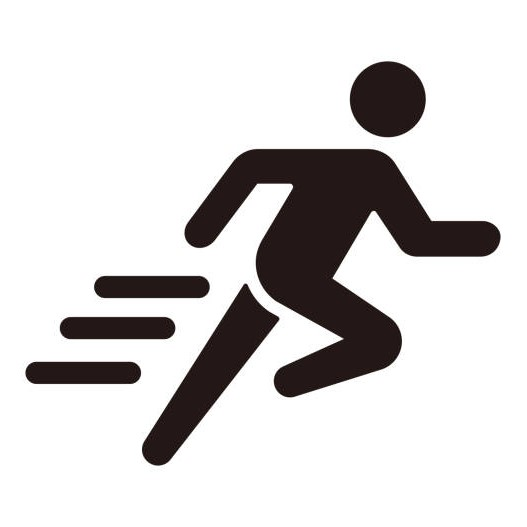
\includegraphics[width = \linewidth]{src/1_kreislauf/images/joggen_piktogramm.jpg}
    \end{minipage}
    \begin{minipage}{0.64\linewidth}
        \begin{itemize}
            \item 5-10 Minuten Joggen
            \item 3x 1 Min Sprint + 1 Min locker
            \item 30s Sprungvarianten einbauen
        \end{itemize}
    \end{minipage}

    \subsection{Seilspringen}
    \begin{minipage}{0.34\linewidth}
        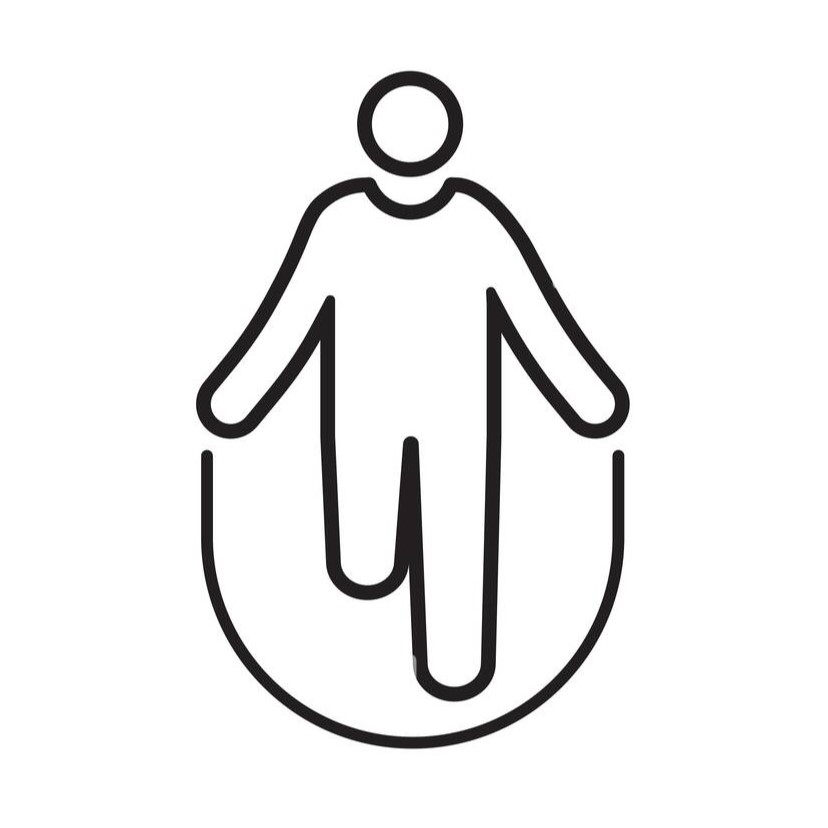
\includegraphics[width = \linewidth]{src/1_kreislauf/images/seilspringen_piktogramm.jpg}
    \end{minipage}
    \begin{minipage}{0.64\linewidth}
        \begin{itemize}
            \item 
        \end{itemize}
    \end{minipage}

\begin{itemize}
    \item Seilspringen
    \item Treppenlaufen
\end{itemize}